\documentclass[10pt]{beamer}
\usepackage{etex}
\usetheme[
%%% options passed to the outer theme
%    progressstyle=fixedCircCnt,   %either fixedCircCnt, movCircCnt, or corner
%    rotationcw,          % change the rotation direction from counter-clockwise to clockwise
%    shownavsym          % show the navigation symbols
  ]{AAUsimple}
  
% If you want to change the colors of the various elements in the theme, edit and uncomment the following lines
% Change the bar and sidebar colors:
%\setbeamercolor{AAUsimple}{fg=red!20,bg=red}
%\setbeamercolor{sidebar}{bg=red!20}
% Change the color of the structural elements:
%\setbeamercolor{structure}{fg=red}
% Change the frame title text color:
%\setbeamercolor{frametitle}{fg=blue}
% Change the normal text color background:
%\setbeamercolor{normal text}{fg=black,bg=gray!10}
% ... and you can of course change a lot more - see the beamer user manual.

\usepackage[utf8]{inputenc}
\usepackage[spanish]{babel}
\usepackage[T1]{fontenc}
% Or whatever. Note that the encoding and the font should match. If T1
% does not look nice, try deleting the line with the fontenc.
\usepackage{helvet}
\usepackage{graphics}
\usepackage{color}
\usepackage[all]{xy}


\usepackage{graphicx}
\graphicspath{ {AAUgraphics/} }

% colored hyperlinks
\newcommand{\chref}[2]{%
  \href{#1}{{\usebeamercolor[bg]{AAUsimple}#2}}%
}

\title{Operadores de cruce y reemplazo de individuos}

\subtitle{Computación evolutiva}  % could also be a conference name

\date{7 de octubre de 2015}

\author{
David Atienza \and
Guillermo Delgado \and
Javier López \and \\
Rubén Martín \and
Álvaro Muñoz \and
Gustavo Puig
}

% - Give the names in the same order as they appear in the paper.
% - Use the \inst{?} command only if the authors have different
%   affiliation. See the beamer manual for an example

\institute[
%  {\includegraphics[scale=0.2]{aau_segl}}\\ %insert a company, department or university logo
%  Dept.\ of Electronic Systems\\
%  Aalborg University\\
%  Denmark
] % optional - is placed in the bottom of the sidebar on every slide
{% is placed on the bottom of the title page
 Departamento de Inteligencia Artificial
  
  %there must be an empty line above this line - otherwise some unwanted space is added between the university and the country (I do not know why;( )
}

% specify a logo on the titlepage (you can specify additional logos an include them in 
% institute command below
\pgfdeclareimage[height=2.75cm]{titlepagelogo}{AAUgraphics/logocei.png} % placed on the title page
\titlegraphic{% is placed on the bottom of the title page
  \pgfuseimage{titlepagelogo}
%  \hspace{1cm}\pgfuseimage{titlepagelogo2}
}

\setcounter{tocdepth}{1}

\begin{document}
% the titlepage
{%\aauwavesbg%
\begin{frame}[plain,noframenumbering] % the plain option removes the header from the title page
  \titlepage
\end{frame}}
%%%%%%%%%%%%%%%%

% TOC
\begin{frame}{Índice}{}
\tableofcontents
\end{frame}
%%%%%%%%%%%%%%%%

\section{Algoritmos genéticos}

\begin{frame}{Algoritmos genéticos}{Funcionamiento general}
	\resizebox{\textwidth}{!}{
		\xymatrix{
		*+++[F]\txt{Generar población inicial} \ar[d] &	\\
		*+++[F]\txt{Evaluar individuos de la población} \ar[r] \ar[d] & 	*+++[F]\txt{Aplicar selección, cruce y/o mutación} \ar[d] \\
		*+++++[o][F]\txt{Población final: solución} & *+++[F]\txt{Generar una nueva población} \ar@(r,d)[lu] \\
		}
	}
\end{frame}

\begin{frame}{Algoritmos genéticos}{Operadores cruce y reemplazo}

	\begin{itemize}
		\item Operador cruce:
			\begin{itemize}
				 \item Obtener descendientes a partir de los padres
				 \item Los nuevos individuos tienen parte del genotipo de los padres
				 \item Diferentes métodos entre alfabeto finito y codificación real
			\end{itemize}
		\item Operador reemplazo:
			\begin{itemize}
				\item Reemplazar individuos de la antigua población por los nuevos individuos
			\end{itemize}
	\end{itemize}
\end{frame}

\begin{frame}{Exploración y explotación}
		\textbf{OBJETIVO:} Todo algoritmo genético necesita establecer un equilibrio entre dos factores aparentemente opuestos:
	\begin{itemize}

		\item Exploración:
			\begin{itemize}
				 \item Diversidad de soluciones
				 \item Explorar todo el espacio de soluciones para localizar zonas prometedoras
				 \item Evitar óptimos locales
			\end{itemize}
		\item Explotación:
			\begin{itemize}
				\item Convergencia de soluciones
				\item Centrar la búsqueda en regiones exploradas para mejorar las soluciones encontradas
				\item Evitar la búsqueda aleatoria 
			\end{itemize}
	\end{itemize}

\end{frame}

\begin{frame}{Exploración y explotación}
	\begin{center}
		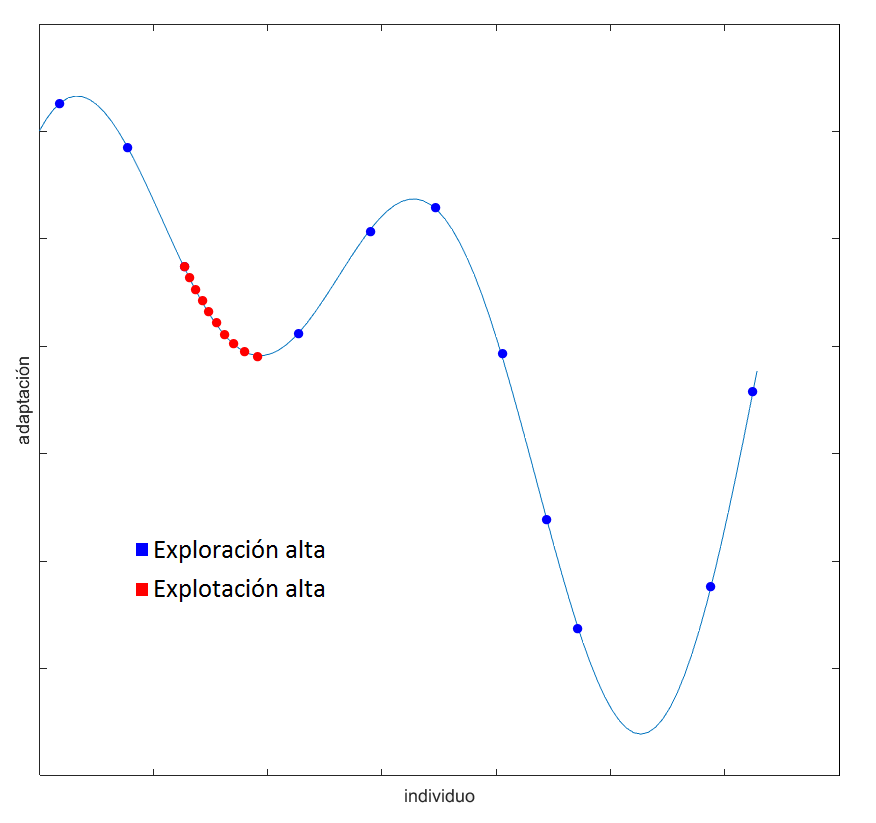
\includegraphics[width=\textwidth,height=0.8\textheight,keepaspectratio]{exploracion_explotacion}
	\end{center}
\end{frame}

\begin{frame}{Exploración y explotación}
	Existen diversas formas de variar la exploración y la explotación: 
	
	\begin{itemize}

		\item Operador mutación: Aumenta la exploración.

		\item Operador selección: Elegir a los mas aptos aumenta la explotación
		
		\item Operador cruce: Descendientes con genotipo similar a los padres aumenta la explotación
		
		\item Reemplazo: Eliminar a los individuos menos adaptados aumenta la explotación.

	\end{itemize}
	\begin{center}
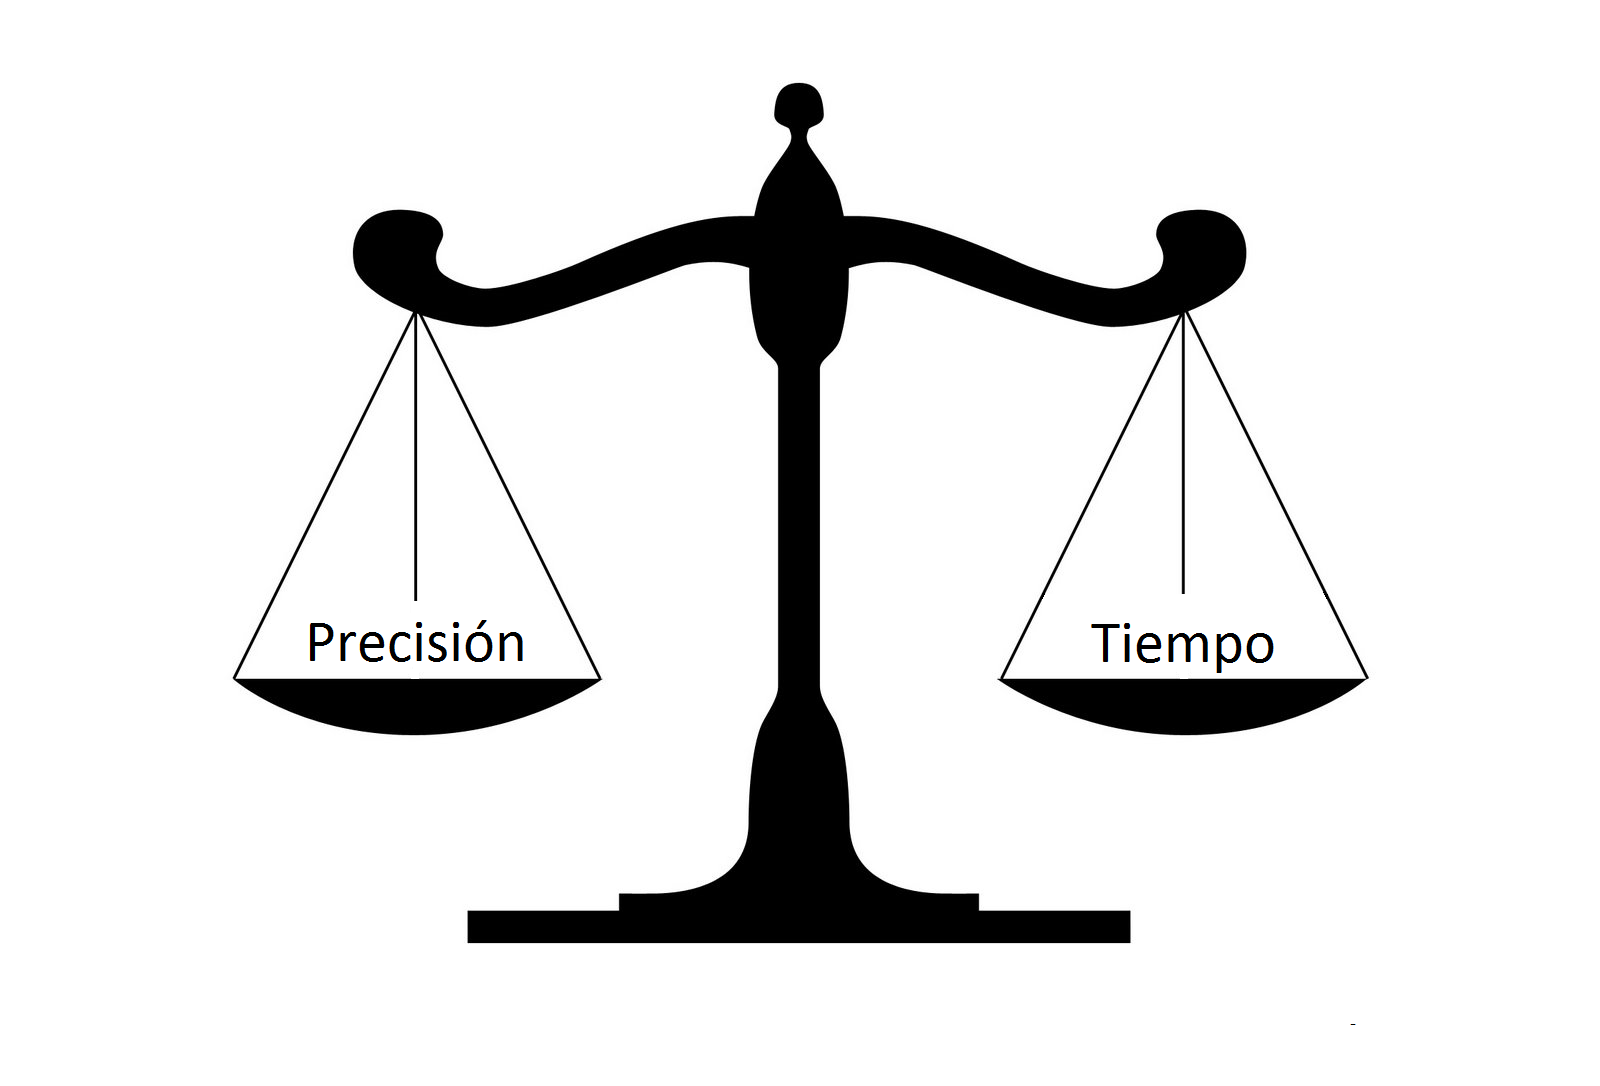
\includegraphics[width=170pt]{balanza}
	\end{center}
\end{frame}

\section{Operadores de cruce con alfabeto finito}

\subsection{Tipos de operadores}

\begin{frame}{Operadores de cruce con alfabeto finito I}{Conceptos básicos}
	\begin{itemize}
		\item Los puntos de la función a optimizar utilizan un \textbf{alfabeto finito}: 
			$$ A = \{0, 1, ..., m\} $$
		\item Los \textbf{individuos} de la población son los puntos del espacio de búsqueda :
			$$ c_1, c_2, ..., c_l \quad\quad \forall c_k \in A, k \in \{1, 2, ..., l\} $$
		\item Individuos seleccionadas de la \textbf{población} (con probabilidad $\boldsymbol{p_c}$): \\
			\begin{center}
				Individuos progenitores o \textbf{padres}
			\end{center}
		\item Individuos generados por el operador: \\
			\begin{center}
				Individuos \textbf{descendientes}
			\end{center}
	\end{itemize}
\end{frame}

\begin{frame}{Operadores de cruce con alfabeto finito II}{Operador de cruce ordinario U operador basado en un punto}
	
	\begin{itemize}
		\item Padres:
			$$ 01010 \quad y \quad 10101 $$
		
		\item Lugar de cruce $ k \in [1, 5]  $:
				$$\xymatrix@=5pt{
					 010  &  10 \ar[dd] & \\
					  & & k = 3 \\
					 101  &  01  \ar[uu] &\\
				} $$
		\item Descendientes:
		
			$$ 01001 \quad y \quad 10110 $$
	\end{itemize}
	\end{frame}

\begin{frame}{Operadores de cruce con alfabeto finito III}{Operador de cruce basado en dos puntos}
		\begin{itemize}
			\item Padres:
			$$ 01010 \quad y \quad 10101 $$
			
			\item Lugares de cruce $ k, k' \in [1, 5] $:

				$$\xymatrix@=5pt{
					01 & 01 \ar[dd]  &  0  & \\
					& & & k = 2 \quad y \quad k' = 4 \\
					10 & 10 \ar[uu] & 1   &\\
				} $$
			
			\item Descendientes:
				$$ 01100 \quad y \quad 10011 $$
		\end{itemize}
\end{frame}

\begin{frame}{Operadores de cruce con alfabeto finito IV}{Operador de cruce uniforme}
			\begin{itemize}
				\item Padres:
				$$ 01010 \quad y \quad 10101 $$
				
				\item Máscara de cruce aleatoria: $$ m = 01001 $$

				\item ¿Cómo aplicar la máscara?
					
					\begin{itemize}
						\item Descendiente 1: \\\begin{center}
							 $a_i$ si $m_i$ es 0, $b_i$ si $m_i$ es 1
						\end{center}
						\item Descendiente 2: \\ \begin{center}$a_i$ si $m_i$ es 1, $b_i$ si $m_i$ es 0	\end{center}
					\end{itemize}
					
							
				\item Descendientes:
				$$ 00011 \quad y \quad 11100 $$
			\end{itemize}
\end{frame}

%\begin{frame}{Operadores de cruce con alfabeto finito V}{Operador de cruce basado en la función objetivo}
%		\begin{itemize}
%			\item Modificación del cruce uniforme. 
%			
%			\item Ahora se tiene en cuenta la función de adaptación de los padres.
%			
%			\item ¿Cómo aplicar la máscara?
%				$$ X \sim \operatorname{Bern} \left({p}\right)$$
%
%				$$ f(x) = p^x(1-p)^{1-x} \quad \text{con} \quad x = \{0,1\}$$
%
%				$$ p = \frac{f(I_i)}{f(I_i)+f(Ij)} $$	
%		\end{itemize}
%\end{frame}
%
%\begin{frame}{Operadores de cruce con alfabeto finito VI}{Operador de cruce basado en el enfriamiento simulado}
%	\begin{itemize}
%		\item Umbral de energía $\theta_c$.
%		\item La temperatura T decrece lentamente.
%		\item Se elige el bit(i+1)-ésimo se toma del padre opuesto del bit i-ésimo con probabilidad (alternancia de progenitores):
%			$$e^{\frac{-\theta_c}{T}}$$
%			
%		\item A temperaturas altas, la probabilidad se acerca a 1 (similar al cruce uniforme). 
%		\item A temperaturas bajas, la probabilidad se acerca a 0 (apenas se cambia de progenitor).	
%	\end{itemize}
%\end{frame}

\begin{frame}{Operadores de cruce con alfabeto finito V}{Operador de cruce generalizado}
		\begin{itemize}
			\item Se trabaja con cadenas binarias $ S = \{0,1\}^l$.
			\item Existe una función biyectiva para transformar las cadenas:
				$$ g: S \to \{0, 1, ..., 2^l - 1\}$$
			\item Descendiente 1:
				$$ a' \in g^{-l} ([g(a \wedge b), g(a \lor b)]) $$
			\item Descendiente 2:
				$$ b' \in g^{-l} (g(a) + g(b) - g(a') $$
				
				
		\end{itemize}
		
			\resizebox{\textwidth}{!}{
				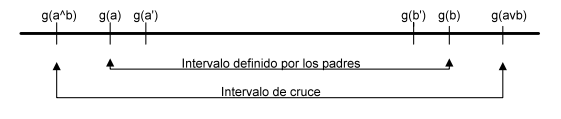
\includegraphics{AAUgraphics/cruce}}
\end{frame}

\begin{frame}{Operadores de cruce con alfabeto finito VI}{Conclusiones}
	\begin{block}{Reflexiones}
	\begin{itemize}
		\setlength\itemsep{1em}
		\item ¿Qué ocurre con el ordenamiento de los genes?
		\item ¿Y si los padres tienen el mismo gen?
		\item ¿Puede llegar a ocurrir que se convierta en una búsqueda aleatoria?
		\item ¿Equilibrio entre exploración y explotación?
		\item ¿Son capaces todos los operadores de encontrar cualquier solución?
		\item ¿Todos los operadores funcionan de forma similar?
	\end{itemize}
\end{block}
\end{frame}


%\subsection{Convergencia con codificación binaria}
%
%\begin{frame}{Convergencia con codificación binaria}{}
%	\begin{block}{Modelo de Holland}
%	\begin{enumerate}
%		\item La población debe ser infinita.
%		\item La función de evaluación debe reflejar el grado de utilidad de una solución.
%		\item Los genes dentro de un cromosoma no deben interactuar entre sí significativamente.
%	\end{enumerate}
%
%	\end{block}
%	
%		\begin{block}{\alert{¡¡Errores estocásticos!!}}
%				\begin{itemize}
%					\item Genes fijos.
%					\item En algoritmia genética, el tamaño sí importa.
%				\end{itemize}
%			\end{block}	
%\end{frame}

%\begin{frame}{Convergencia con codificación binaria}
%	\begin{block}{Problemas paradójicos}
%		\begin{itemize}
%			\item Los operadores de cruce clásicos no funcionan.
%			\item Funciones de Walsh
%			\item Conocer  la dificultad del problema  de optimización
%		\end{itemize}
%	\end{block}	
%\end{frame}


\section{Operadores de cruce con codificación real}

\begin{frame}{Operadores de cruce con codificación real}
	\begin{center}
		\huge ¿Que ocurre si usamos un método de cruce de los explicados anteriormente?
	\end{center}
		
\end{frame}

\begin{frame}{Operadores de cruce con codificación real}

		\begin{itemize}
			\item Supongamos que tenemos lo siguiente:
			\begin{itemize}
				\item $a=a_{1} , a_{2}, ... , a_{l}$ y $b=b_{1} , b_{2}, ... , b_{l}$ 
				\\$a_{i},b_{i} \in \mathbb{R}$, $\forall i \in \{1, ... , l\}$
			\end{itemize}
			\item lo cruzamos y obtenemos:
			\begin{itemize}
				\item  $c=c_{1} , c_{2}, ... , c_{l}$
				\\$c_{i} \in \{ a_{1}, ... , a_{l},b_{1}, ... , b_{l} \}$, $\forall i \in \{1, ... , l\}$
			\end{itemize}
			
		\end{itemize}
		
		\begin{center}
			\vspace{5mm}
			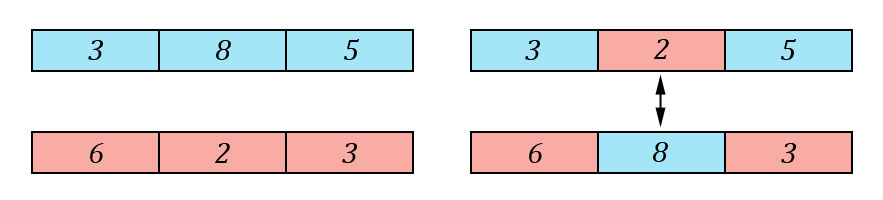
\includegraphics[width=10cm]{crucereal}
		\end{center}
		

\end{frame}

\subsection{Operador de cruce plano}

\begin{frame}{Operador de cruce plano (BLX)}{Radcliffe}
	\begin{itemize}
		\item A partir de 2 progenitores generamos 2 descendientes
		\item Utiliza un intervalo de números reales (intervalo de cruce)
		\item Se escoge un valor aleatorio dentro del intervalo
		
	\end{itemize}
		\begin{columns}[t]
			\begin{column}{0.4\textwidth}
				\begin{flushright}
					$a=a_{1} , a_{2}, ... , a_{l}$
					\\ $b=b_{1} , b_{2}, ... , b_{l}$ 
				\end{flushright}
			\end{column}
			\begin{column}{0.2\textwidth}
				\begin{center}
					
\includegraphics[width=1cm]{arrow}
				\end{center}
			\end{column}
			\begin{column}{0.4\textwidth}
				\begin{flushleft}
					$c=c_{1} , c_{2}, ... , c_{l}$
					\\ $d=d_{1} , d_{2}, ... , d_{l}$ 
				\end{flushleft}
			\end{column}
	\end{columns}
	
	\begin{center}
		$C_{i}=[min(a_i,b_i) , max(a_i,b_i)]$
		
		\vspace{5mm}
		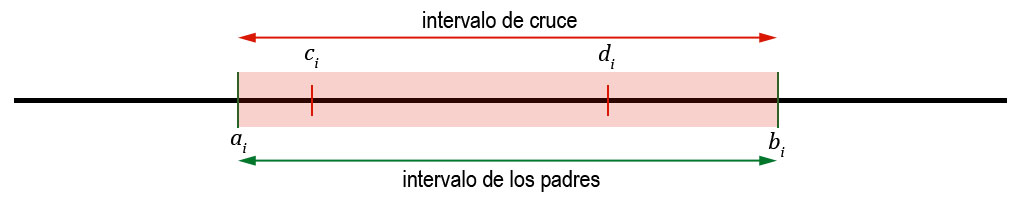
\includegraphics[width=10cm]{cruceplano}
	\end{center}
	

	
	
\end{frame}



\subsection{Operador de cruce lineal}

\begin{frame}{Operador de cruce lineal}{Wright}
		\begin{itemize}
			\item A partir de 2 progenitores generamos 3 descendientes
			\item Se escoge en el primer caso el valor intermedio del intervalo 
			\item Los otros individuos se escogen fuera del intervalo de los progenitores, concretamente se alejan la misma distancia que la que hay al centro
		\end{itemize}
		\begin{columns}[t]
			\begin{column}{0.4\textwidth}
				\begin{flushright}
					$a=a_{1} , a_{2}, ... , a_{l}$
					\\ $b=b_{1} , b_{2}, ... , b_{l}$ 
				\end{flushright}
			\end{column}
			\begin{column}{0.2\textwidth}
				\begin{center}
					
\includegraphics[width=1cm]{arrow}
				\end{center}
			\end{column}
			\begin{column}{0.4\textwidth}
				\begin{flushleft}
					$c=c_{1} , c_{2}, ... , c_{l}$
					\\ $d=d_{1} , d_{2}, ... , d_{l}$ 
					\\ $e=e_{1} , e_{2}, ... , e_{l}$ 
				\end{flushleft}
			\end{column}
		\end{columns}
		
		\begin{center}
			$c_{i}= \frac {a_i+b_i} {2}$
			\\$d_i = 1.5 \cdot a_i-0.5 \cdot b_i$
			\\$e_i = -0.5 \cdot a_i+1.5 \cdot b_i$
			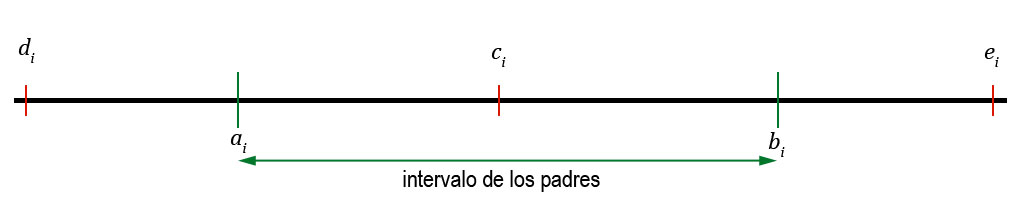
\includegraphics[width=10cm]{crucelineal}
		\end{center}
\end{frame}



\subsection{Operador de cruce combinado}

\begin{frame}{Operador de cruce combinado (BLX-a)}
	\begin{itemize}
		\item A partir de 2 progenitores generamos 2 descendientes
		\item Se escoge un valor aleatorio dentro del intervalo de cruce
		\item Generamos un intervalo que puede ser mas grande que el intervalo de los progenitores dado por $\alpha$
	\end{itemize}
	\begin{columns}[t]
		\begin{column}{0.4\textwidth}
			\begin{flushright}
				$a=a_{1} , a_{2}, ... , a_{l}$
				\\ $b=b_{1} , b_{2}, ... , b_{l}$ 
			\end{flushright}
		\end{column}
		\begin{column}{0.2\textwidth}
			\begin{center}
				
\includegraphics[width=1cm]{arrow}
			\end{center}
		\end{column}
		\begin{column}{0.4\textwidth}
			\begin{flushleft}
				$c=c_{1} , c_{2}, ... , c_{l}$
				\\ $d=d_{1} , d_{2}, ... , d_{l}$ 
			\end{flushleft}
		\end{column}
	\end{columns}
	
	\begin{center}
		$C_{i}=[a_i - \alpha I , b_i - \alpha I]$
		
		\vspace{5mm}
		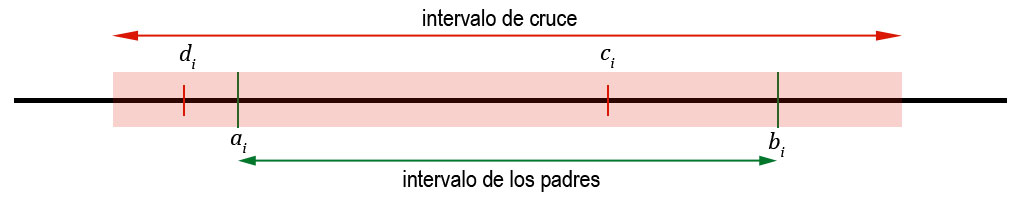
\includegraphics[width=10cm]{crucecombinado}
	\end{center}	
\end{frame}




\subsection{Operador de cruce morfológico}

\begin{frame}{Operador de cruce morfológico (MMX)}
	\begin{itemize}
		\item A partir de un número n impar de progenitores obtenemos dos descendientes
		\item Se genera un intervalo de cruce que \textbf{depende de la diversidad genética} 
		\item Los descendientes se generan eligiendo números aleatorios dentro del intervalo de cruce
		\item Se normaliza el dominio
	\end{itemize}
	
	\begin{center}
		%\vspace{5mm}
		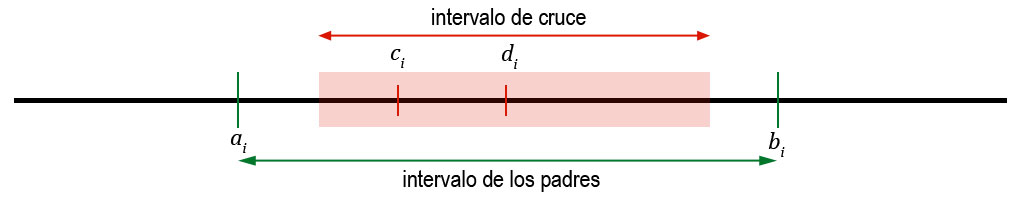
\includegraphics[width=10cm]{crucemorfologico}
		\vspace{3mm}
		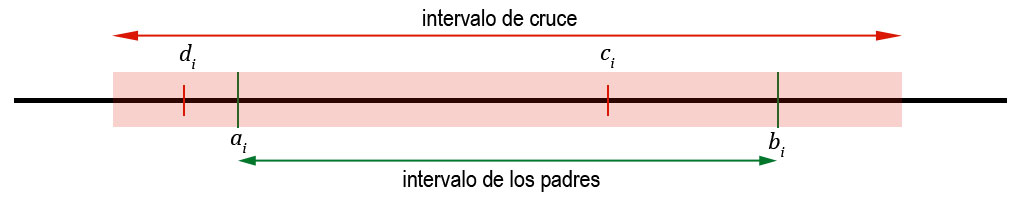
\includegraphics[width=10cm]{crucecombinado}
		
	\end{center}	
\end{frame}

\begin{frame}{Operador de cruce morfológico (MMX)}
	\begin{itemize}

		\item Se ejecutan los siguientes pasos:
		\begin{enumerate}
			\item Cálculo de la medida de la diversidad genética
			\item Cálculo de los intervalos de cruce
			\item Obtención de la descendencia
		\end{enumerate}
	\end{itemize}
	
\end{frame}


\subsubsection{Cálculo de la medida de la diversidad genética}

% INTRODUCCIÓN:
\begin{frame}{Operador de cruce morfol\'ogico}{Medida de la Diversidad Gen\'etica}
	\textbf{Definici\'on:} an\'alis de la tendencia de la evoluci\'on genen\'etica para deducir din\'amicamente que t\'ecnicas evolutivas aplicar.
	
	\begin{itemize}
		\item T\'ecnicas:
		\begin{enumerate}
			\item Explotaci\'on.
			\item Exploraci\'on.
		\end{enumerate}
	\end{itemize}
	
	\textbf{OBJETIVO:} dado un subconjunto de una poblaci\'on de $\lambda$ individuos, estudiar cu\'an grande es la variedad gen\'etica con respecto al individuo con \underline{caracter\'isticas medias}.
	
	\textbf{?`C\'OMO SE ANALIZA?} Utilizando Morfolog\'ia Matem\'atica aplicada a im\'agenes binarias $\rightarrow$  \underline{Gradiente Morfol\'ogico}.
	
\end{frame}

% CONCEPTO DE GRADIENTE
\begin{frame}{Operador de cruce morfol\'ogico}{Medida de la Diversidad Gen\'etica}
	\begin{center}
		CONCEPTO DE GRADIENTE:
		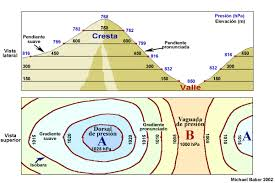
\includegraphics[width=10cm]{gradiente_altura}
	\end{center}
\end{frame}

%APLICACIÓN DE GRADIENTE MORFOLOGICO SOBRE IMAGENES
\begin{frame}{Operador de cruce morfol\'ogico}{Medida de la Diversidad Gen\'etica}
	\begin{center}
		\underline{\textbf{MORFOLOG\'IA MATEM\'ATICA SOBRE IM\'AGENES: }}
		
		\begin{itemize}
			\item \textbf{MORFOLOG\'IA} $\rightarrow$ \textit{MORFOS} $\rightarrow$ \emph{forma}.
			\item \textbf{VISION ARTIFICIAL} $\rightarrow$ Gradiente Morfol\'ogico \par
			$\rightarrow$ segmentaci\'on de im\'agenes para obtenci\'on de formas.
		\end{itemize}
		
		\fbox{
			\begin{tabular}{ c c c }
				Original & Normalizado/Binarizado & Grad. Morfol\'ogico \\ 
				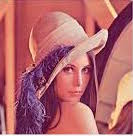
\includegraphics[width = 3cm]{rb_original} & 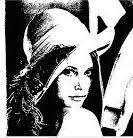
\includegraphics[width = 3cm]{rb_binarizado} & 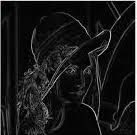
\includegraphics[width = 32mm]{rb_gradmorf}
			\end{tabular}}
			
		\end{center}
	\end{frame}
	
	%EXPLICACIÓN MATEMÁTICA DEL GRADIENTE MORFOLÓGICO SOBRE IMAGEN BIDIMENSIONAL [1]
	
	\begin{frame}{Operador de cruce morfol\'ogico}{Medida de la Diversidad Gen\'etica}
		\begin{center}
			\underline{\textbf{MATEM\'ATICAMENTE SOBRE UNA IMAGEN BIDIMENSIONAL:}}\\
			\fbox{Ingenier\'ia inversa: $g_{m}(f) = dilatation(f) - erotion (f)$}
			\begin{itemize}
				\item DILATACI\'ON: $(f \bigoplus b)(s,t) = \max \{f(s-x, t-y)+b(x,y)$ : $(s-x, t-y) \in D_{f} ; (x,y) \in D_{b} \} $
			\end{itemize}
			
			\fbox{
				\begin{tabular}{ c c c }
					Original & Elmnt. Estructurante & Dilataci\'on \\ 
					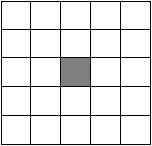
\includegraphics[width = 2cm]{matriz_pixel} & 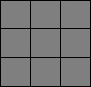
\includegraphics[width = 1cm]{elemento_estructurante} & 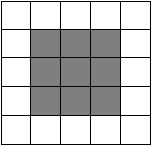
\includegraphics[width = 2cm]{matriz_dilatada} 
				\end{tabular}}
				
				\begin{itemize}
					\item Si nuestro objetivo es obtener la m\'axima variaci\'on, el estructurante debe ser nulo para no limitar la dilataci\'on:
				\end{itemize}
				
				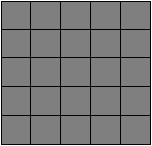
\includegraphics[width = 2cm]{matriz_dilatada_sin_estructurante} 
				
			\end{center}
		\end{frame}
		
		%EXPLICACIÓN MATEMÁTICA DEL GRADIENTE MORFOLÓGICO SOBRE IMAGEN BIDIMENSIONAL [2]
		
		\begin{frame}{Operador de cruce morfol\'ogico}{Medida de la Diversidad Gen\'etica}
			\begin{center}
				\underline{\textbf{PARA EL CASO DE LA EROSI\'ON:}}
				
				\begin{itemize}
					\item $(f \ominus b)(s,t) = \min \{f(s+x, t+y)-b(x,y)$ : $(s+x, t+y) \in D_{f} ; (x,y) \in D_{b} \} $
				\end{itemize}
				
				\fbox{
					\begin{tabular}{ c c c }
						Original & Elmnt. Estructurante & Dilataci\'on \\ 
						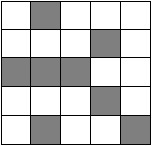
\includegraphics[width = 2cm]{matriz_para_erosion} & 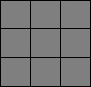
\includegraphics[width = 1cm]{elemento_estructurante} & 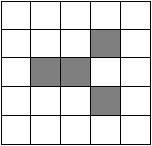
\includegraphics[width = 2cm]{matriz_erosionada} 
					\end{tabular}}
					
					\begin{itemize}
						\item Si nuestro objetivo es obtener la m\'axima variaci\'on, el estructurante debe ser nulo para no limitar la erosi\'on:
					\end{itemize}
					
					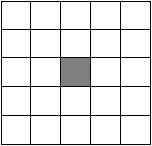
\includegraphics[width = 2cm]{matriz_pixel} 
					
				\end{center}
			\end{frame}
			
			
			%EXTRAPOLAMOS A CASO UNIDIMENSIONAL
			
			\begin{frame}{Operador de cruce morfol\'ogico}{Medida de la Diversidad Gen\'etica}
				\begin{center}
					\underline{\textbf{EXTRAPOLANDO A NUESTRO CASO:}}
					
					$ G[matriz progenitora] = \left(\begin{array}{cccc}
					a_{0,0}   & a_{0,1} & \ldots &a_{0,l-1} \\
					a_{1,0}   & a_{1,1} & \ldots &a_{1,l-1} \\
					a_{2,0}   & a_{2,1} & \ldots &a_{2,l-1} \\
					a_{3,0}   & a_{3,1} & \ldots &a_{3,l-1} \\
					\vdots  & \vdots & \ldots &\vdots \\
					a_{n,0}   & a_{n,1} & \ldots &a_{n,l-1} 
					\end{array} \right)$ \par
					donde n $(n \leqslant \lambda)$ es el N. de progenitores y l la longitud de cada cromosoma.
					
					\begin{itemize}
						\item Maximizar informaci\'on $\rightarrow$ analizar la evoluci\'on de los genes en particular \underline{(y no los cromosomas/individuos en general)}.
					\end{itemize}
					\fbox{$f_{0} = (a_{0,0} ,  a_{1,0} a_{2,0}  a_{3,0} \ldots a_{n-1,0})$}
				\end{center}
			\end{frame}
			
			
			%CASO PARTICULAR
			
			\begin{frame}{Operador de cruce morfol\'ogico}{Medida de la Diversidad Gen\'etica}
				
				\underline{\textbf{CASO PARTICULAR:}}
				\begin{itemize}
					\item Si tomamos $n = 5$ con cardinal $\left[1,6\right]$; $f_{0} = (6, 2, 4, 1, 3, 5)$.
				\end{itemize}
				Nuestro inter\'es es averiguar la desviaci\'on con respecto el \underline{gen que ocupa la posici\'on media.}\\
				Teniendo en cuenta que nuestro \underline{elemento estructurante} es \underline{nulo} no ofrece restricciones a la dilataci\'on.
				\begin{itemize}
					\item El valor m\'aximo dilatado que podemos obtener ser\'a 6.
					\item Del mismo modo, la menor de las erosiones de nuestra muestra ser\'a el menor de todos los valores: 1.
				\end{itemize}
				
				\begin{center}
					\underline{\textbf{CONCLUSI\'ON:}} $g_{m}(f_{i}) = max(f_{i})- min(f_{i})$.
				\end{center}
				
			\end{frame}
			
			
			%CONCLUSIONES
			
			\begin{frame}{Operador de cruce morfol\'ogico}{Medida de la Diversidad Gen\'etica}
				\begin{center}
					\underline{\textbf{AN\'ALISIS DE RESULTADOS:}}
				\end{center}
				
				\textbf{Si $g_{m}(f_{i})$ es muy elevado:}
				\begin{itemize}
					\item Los genes de en la posici\'on i de nuestro progenitores toman valores dispersos $\rightarrow$ nuestra poblaci\'on sobreexplora el espacio de b\'usqueda.
					\item  Debemos aplicar cruces que fomenten la explotaci\'on $\rightarrow$ los genes (i) de sus hijos deben tomar valores m\'as centrados en la media de la imagen.
				\end{itemize}
				
				\textbf{Si $g_{m}(f_{i})$ es muy peque\~{n}o:}
				\begin{itemize}
					\item Los genes de en la posici\'on i de nuestro progenitores toman valores cercanos $\rightarrow$ nuestra poblaci\'on sobreexplota el espacio de b\'usqueda.
					\item  Debemos aplicar cruces que fomenten la exploraci\'on $\rightarrow$ los genes (i) de sus hijos deben tomar valores m\'as separados de la media de la imagen.
				\end{itemize}
				
			\end{frame}

\subsubsection{Cálculo de los intervalos de cruce}

\begin{frame}{Cálculo intervalos de cruce}
	\begin{itemize}
		\item Buscamos los intervalos $C_{i}$
		\item Estos intervalos dependerán de una función $\varphi:\mathbb{R}\rightarrow\mathbb{R}$ denominada \textbf{función de exploración/explotación}.
		\item Sean $g_{imax}$ gen máximo y $g_{imin}$ gen mínimo:
		\begin{itemize}
			\item $g_{imax}=\underbrace{(f_{i}\oplus b)(E(n/2)+1)}_{Dilatación f_{i} en el punto medio}-\varphi(g_{i}) = máx(f_{i})-\varphi(g_{i})$
			\item $g_{imin}=\underbrace{(f_{i}\ominus b)(E(n/2)+1)}_{Erosión f_{i} en el punto medio}+\varphi(g_{i}) = mín(f_{i})+\varphi(g_{i})$
		\end{itemize}
		\item Definiremos los intervalos de cruce: $C_{i}=[g_{imin},g_{imax}]$ con i=0,...,l-1.
	\end{itemize}
\end{frame}
\begin{frame}{Cálculo intevalos de cruce}
	La función de exploración/explotación,FEE,es crucial en la determinación de los intervalos.
	\begin{itemize}
		\item Si $\varphi(g_{i})=0,\forall g_{i}$ entonces:
		\begin{itemize}
			\item Los intervalos de cruce serán de la forma $C_{i}=[mín(f_{i}),máx(f_{i})]$(\textit{intervalo definido por los padres} o \textit{intervalo de referencia}).
			\item Genera únicamente individuos pertenecientes al intervalo de cruce definido por los padres.
			\item Aplica únicamente técnicas de explotación $\rightarrow$convergencia prematura.
		\end{itemize}
		\item La FEE al depender de $g_{i}$ nos permite establecer una regla que distinga si debemos optar por la exploración o la explotación.
	\end{itemize}
\end{frame}
\begin{frame}{Cálculo intervalos de cruce}
	Estudio casos:
	\begin{itemize}
		\item Si los valores que toma un determinado gen son muy similares(convergencia hacia un punto):
		\begin{itemize}
			\item $g_{i}$ estará próximo a 0.
			\item La FEE deberá permitir la expansión del intervalo para evitar la convergencia a un punto que no sea el óptimo(exploración).
			\item $\varphi(g_{i})$ deberá tomar valores negativos para expandir el intervalo.
		\end{itemize}
		\item Si los valores son muy distintos(dispersión de la población en el espacio de búsqueda):
		\begin{itemize}
			\item $g_{i}$ estará próximo a 1.
			\item La FEE deberá permitir la expansión del intervalo para evitar la convergencia a un punto que no sea el óptimo(exploración).
			\item $\varphi(g_{i})$ deberá tomar valores positivos para estrechar el intervalo.
		\end{itemize}
	\end{itemize}
\end{frame}

\begin{frame}{Convergencia con codificación binaria}
	\resizebox{\textwidth}{!}{
		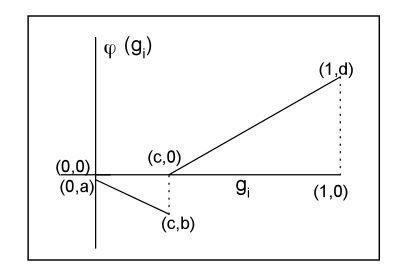
\includegraphics{AAUgraphics/FuncionFEE}}
\end{frame}

\begin{frame}{Cálculo intervalos de cruce}
	Resumen de las condiciones que debe cumplir $\varphi(g_{i})$:
	\begin{itemize}
		\item 1- Debe proporcionar valores positivos para valores elevados de $g_{i}$ y negativos para valores próximos a 0.
		\item 2- Coste computacional bajo.
		\item 3- El dominio debe ser el intervalo real [0,1]
		\item 4- Se debe cumplir que $g_{imin}\leq g_{imax}$
		\item 5- $\varphi(g_{i})\neq 0$
	\end{itemize}		
\end{frame}


\subsubsection{Cálculo de la descendencia}
\begin{frame}{Operadores de cruce con codificación real}{Cálculo de la descendencia}
	\begin{itemize}
		\item Una vez conocidos los intervalos de cruce $C_{i}$ de cada gen, podemos calcular nuevos individuos.
		\item Crearemos dos individuos, $o = (o_{0},.., o_{l-1})$ y $o' = (o'_{0},.., o'_{l-1}) $.
		\item Como cada gen tiene un intervalo de cruce diferente, se debe aplicar el siguiente procedimiento por cada gen:
		\begin{enumerate}
			\item $o_{i}$ se escoge aleatoriamente en el intervalo de cruce $C_{i}$.
			\item $o'_{i}$ se calcula con la expresión: \begin{equation*}
				o'_{i} = (min(f_{i}) + max(f_{i})) - o_{i}
			\end{equation*}
		\end{enumerate}
		
		\item Se demuestra que $g_{imin} \leq o'_{i} \leq g_{imax}$.
		\item $o_{i}$ y $o'_{i}$ se encuentran equidistantes al centro del intervalo de cruce.
	\end{itemize}
\end{frame}



\subsubsection{Coste computacional del cruce morfológico}

\begin{frame}{Operadores de cruce con codificación real}{Coste computacional del cruce morfológico}
Algunas consideraciones iniciales:
	\begin{itemize}
		\item Es importante asegurarse de que el coste computacional del cruce no sea demasiado elevado $\Rightarrow$ se repite muchas veces.
		\item La multiplicación es una operación más costosa que una suma / resta.
		\item Repetiremos el proceso de creación de $o_{i}$ y $o'_{i}$ una vez por cada gen, es decir, $l$ veces. Ese proceso debería ser lo menos costoso posible.
		\item Estamos realizando el mismo proceso en los $l$ genes $\Rightarrow$ fácilmente paralelizable en un ordenador con $l$ procesadores.
	\end{itemize}
\end{frame}


\begin{frame}{Operadores de cruce con codificación real}{Coste computacional del cruce morfológico}
Podemos dividir el proceso de cruce en tres partes, que se deben repetir en cada gen:
	\begin{enumerate}
		\item En primer lugar se calcula el gradiente morfológico, $g = max(f_{i}) - min(f_{i})$.
			\begin{itemize}
				\item Para calcular el valor máximo / mínimo, necesitamos realizar $n$ sumas / restas.
			\end{itemize}
		\item Posteriormente, se calcula el intervalo $[g_{imin}, g_{imax}]$.
			\begin{itemize}
				\item $g_{imin} = max(f_{i}) - \varphi(x)$
				\item $g_{imax} = min(f_{i}) + \varphi(x)$
				\item Calcular $\varphi(x)$ supone una multiplicación y una suma.
			\end{itemize}
			
		\item Por último, se calculan los descendientes $o_{i}$ y $o'_{i}$.
			\begin{itemize}
				\item $o'_{i} = (min(f_{i}) + max(f_{i})) - o_{i}$
			\end{itemize}
	\end{enumerate}
	
	\begin{itemize}
		\item En total se realizan $2n + 6$ sumas y $1$ multiplicación por cada gen.
	\end{itemize}
\end{frame}

\section{Reemplazo de individuos}
\begin{frame}{Reemplazo de individuos}
	\begin{itemize}
		\item Se dispone de una población con $\lambda$ individuos y conocemos cómo generar descendientes utilizando el operador de cruce.
		\item Se deben obtener $\lambda$ individuos que formaran parte de la población de la siguiente generación.
		\item ¿Cómo decidir que individuos formarán parte de la siguiente generación?
	\end{itemize}
\end{frame}

\begin{frame}{Reemplazo de individuos}
	\begin{itemize}
		\item La tasa de reemplazamiento generacional, $t_{tg}$, indica el porcentaje de hijos generados respecto al total de la población inicial.
		\item Con $t_{tg} = \lambda^{-1}$, se realiza la sustitución de un individuo de la población por un descendiente.
		\item Aquellos algoritmos genéticos en los que se sustituyen unos pocos individuos se los denomina \textbf{SSGA (\textit{Steady-State Replacement Genetic Algorithms})}.
	\end{itemize}
\end{frame}

\begin{frame}{Reemplazo de individuos}
	Otros reemplazamientos:
	\begin{itemize}
		\item \textbf{Reducción simple}: se realiza un reemplazamiento en bloque, esto es, $t_{tg} = 1$.
		\item \textbf{Reducción elitista de grado $\lambda$}: Se seleccionan a los $\lambda$ mejores individuos a partir de los $\lambda$ individuos iniciales y $\lambda$ descendientes.
		\item \textbf{Algoritmos genéticos modificados}: 
		\begin{itemize}
			\item $r_{1}$ individuos seleccionados por la reproducción para ser cruzados. 			
			\item $r_{2}$ individuos seleccionados para morir.
			\item $\lambda - (r_{1} + r_{2})$ individuos neutros.
			\item Cuanto más adaptado está un individuo tiene más probabilidades de ser seleccionado por la reproducción y menores sus probabilidades de morir
		\end{itemize}
	\end{itemize}
\end{frame}

\begin{frame}{Reemplazo de individuos}{Operadores catastróficos}

Los operadores catastróficos evalúan la convergencia para evitar acabar en un optimo local.

	\begin{itemize}
		\item Se sustituyen individuos de la población por otros nuevos (y generados aleatoriamente).
		\item Se aplican cuando el algoritmo esta convergiendo para escapar de un óptimo local mediante exploración.
		\item No se eliminan a los mejores individuos de la población.
		\item Principales operadores catastróficos:
			\begin{enumerate}
				\item \textbf{Empaquetado}: Todos los individuos con el mismo valor de adaptación son eliminados excepto uno. Evita los individuos repetidos.
				\item \textbf{El día del juicio final}: Solo se conserva el individuo más adaptado. El resto se eliminan.
			\end{enumerate}
		
	\end{itemize}
\end{frame}


{\aauwavesbg
	\begin{frame}[plain,noframenumbering]
		\finalpage{¿Alguna pregunta?}
	\end{frame}}

\end{document}
